\chapter{Semantic Web Architecture}

Semantic web uses URI to identify an existing name or resource, RDF/RDFS and OWL to store new information, and SPARQL to query from the knowledge base. The semantic web stack is already given earlier in Section \ref{subsec:semanticwebstack}. More details are introduced in this chapter.

\section{Uniform Resource Identifier (URI)}

Humans uses symbol and concept to help interpret things and link to objects in real life. This is demonstrated by semiotic triangle as shown in Fig. \ref{fig:semiotictriangle}. The interpretation of ``apple'' is used as an example. The concept is shared among humans in the form of knowledge.

\begin{figure}[htbp]
	\centering
	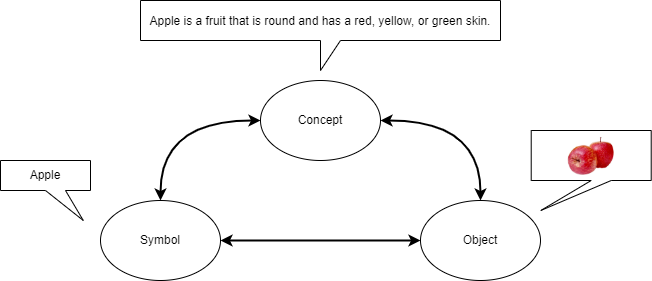
\includegraphics[width=\textwidth]{./chapters/ch-semanticwebarchitecture/figures/semiotic_triangle.png}
	\caption{Semiotic triangle. The symbol is an ``representation'' of a category of items. The concept is the abstracted general properties of an item.}
	\label{fig:semiotictriangle}
\end{figure} 

Uniform resource identifier (URI) is the way to identify a resource of information or knowledge. URI is unique from resource to resource. 

For example, DBpedia gives concept of the apple here: \textit{dbpedia.org/page/Apple}. This is an URL to the web page that contains information of the apple. This URL is an example of URI. In this example, the information can be accessed by HTTP call to the URL.

In semantic web, the URI of a resource identifies an item or a class. Using the URI, the representation (meta data) of the item/class can be accessed. The representation is like the symbol in Fig. \ref{fig:semiotictriangle}, and although it is not a specific instance of the item, it is usually sufficient for us to use the symbol to discuss the item. This is shown in Fig. \ref{fig:identificationflow}.

\begin{figure}[htbp]
	\centering
	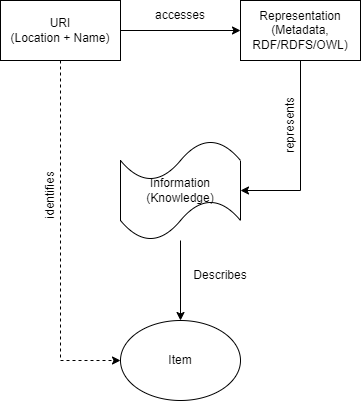
\includegraphics[width=0.6\textwidth]{./chapters/ch-semanticwebarchitecture/figures/identificationflow.png}
	\caption{Identification flowchart.}
	\label{fig:identificationflow}
\end{figure} 

URI shall contain at least two pieces of information: the address (locator), and the identity (name). URI is often ASCII encoded, but it is possible to extend to unicode. The generic syntax is given below, and the URL is a subset of the syntax.
\begin{lstlisting}
scheme:[//authority]path[?query][#fragment]
\end{lstlisting}
where
\begin{itemize}
\item \verb|scheme| specifies the protocol used to access the resource. Common schemes include \verb|http|, \verb|https|, \verb|ftp|, \verb|mailto|, \verb|file|, and \verb|data|. The scheme is followed by a colon \verb|:|.
\item \verb|authority| component is optional and typically includes the user information, host, and port, separated by an at sign \verb|@| and a colon \verb|:|, respectively. The authority is preceded by a double forward slash \verb|//|.
\item \verb|path| identifies the specific resource within the context of the scheme and authority. It is a sequence of segments separated by forward slashes \verb|/|.
\item \verb|query| component is optional and provides additional information that the resource can use for processing. It is a series of key-value pairs separated by an ampersand \verb|&|. The query starts with a question mark \verb|?|.
\item \verb|fragment| component is optional and allows for the identification of a specific part or section within the resource. It is typically used with HTML documents to indicate a specific anchor or location within the page. The fragment starts with a hash sign \verb|#|.
\end{itemize}
More details can be found on
\begin{lstlisting}
https://www.rfc-editor.org/rfc/rfc3986.html#section-3.1
\end{lstlisting}
which happens to be a good example of an URI in https scheme.

\section{Resource Description Framework (RDF)}

The representations of the knowledge shown in \ref{fig:identificationflow} need to be presented in a consistent way. In practice, RDF is introduced to represent knowledge.

Notice that RDF itself is not a programming language. It is the structure using which information is stored. Therefore, it needs a markup language to host the RDF framework. Commonly used markup language the following. There are tools to automatically transfer them from one to another.
\begin{itemize}
  \item RDF/XML: has good compatibility with old machines.
  \item Terse RDF Triple Language (Turtle): easy to use, human-readable.
  \item JSON for Linked Data (JSON-LD): popular in web applications and APIs where JSON-based format is required.
  \item N-Triples: simple, machine-readable format for data exchange between tools.
\end{itemize}
Turtle is very self-explanatory. Unless otherwise mentioned, Turtle is used in this notebook.

\subsection{Triple Representation}

RDF uses ``node-edge-node'' triples to represent knowledge. The triple refers to the combination of: 
\begin{itemize}
  \item Subject
  \item Predicate
  \item Object
\end{itemize}
For example, consider representation of knowledge ``Einstein was born in Ulm''. In RDF, ``Einstein'' is the subject of the knowledge, and ``Ulm'' the object. The predicate is ``has birthPlace'', where ``birthPlace'' is a property assigned to ``Einstein''. The graph representation is given by Fig. \ref{fig:einsteinexp}.
\begin{figure}[htbp]
	\centering
	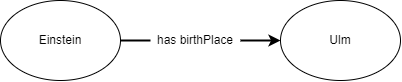
\includegraphics[width=0.6\textwidth]{./chapters/ch-semanticwebarchitecture/figures/einsteinexp.png}
	\caption{Graph representation of triple for knowledge ``Einstein was born in Ulm''.}
	\label{fig:einsteinexp}
\end{figure} 
The RDF is given as follows.
\begin{lstlisting}
@prefix dbo: <http://dbpedia.org/ontology/> .
@prefix dbr: <http://dbpedia.org/resource/> .

dbr:Albert_Einstein dbo:birthPlace dbr:Ulm .
\end{lstlisting}
where \verb|Albert_Einstein| and \verb|Ulm| are defined in \verb|dbpedia.org/resource/| as name and place, and \verb|birthPlace| in \verb|dbpedia.org/ontology/| as an attribute, respectively. To give more details:
\begin{itemize}
  \item \verb|@prefix| keyword is used to define prefixes for namespaces, making it easier to write URIs.
  \item \verb|dbr:Albert_Einstein| is the subject, representing Albert Einstein as a resource in the DBpedia namespace.
  \item \verb|dbo:birthPlace| is the predicate, representing the "birthPlace" property from the DBpedia ontology.
  \item \verb|dbr:Ulm|is the object, representing the city of Ulm as a resource in the DBpedia namespace.
  \item \verb|.| indicates the end of a statement.
\end{itemize}

We use
\begin{lstlisting}
<object> <predicate> <subject> .
\end{lstlisting}
to claim a statement, and
\begin{lstlisting}
<object> <predicate1> <subject1>; <predicate2> <subject2>; <predict3> <subject3> .
\end{lstlisting}
to assign multiple predicates to a subject to avoid repeating the same object in statements.

\subsection{Multi-valued Relation and Blank Node}

It is possible to use multi-valued relations and blank nodes to enforce combining of information. Consider an example given in Fig. \ref{fig:lectureexp}, where the graph is used to demonstrate a lecture taking place at a specific room at given time slot. What if the lecture takes place twice a week, each time at a different location? With the help of multi-valued relations and blank nodes, this can be demonstrated clearly as shown in Fig. \ref{fig:lectureexp2}.
\begin{figure}[htbp]
	\centering
	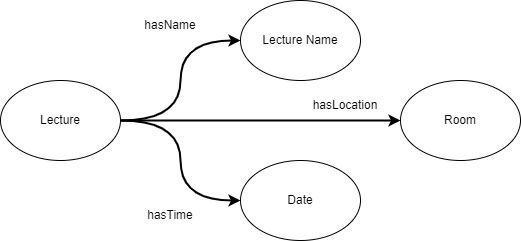
\includegraphics[width=0.6\textwidth]{./chapters/ch-semanticwebarchitecture/figures/lectureexp.png}
	\caption{An example that demonstrate when and where a lecture takes place.}
	\label{fig:lectureexp}
\end{figure}

\begin{figure}[htbp]
	\centering
	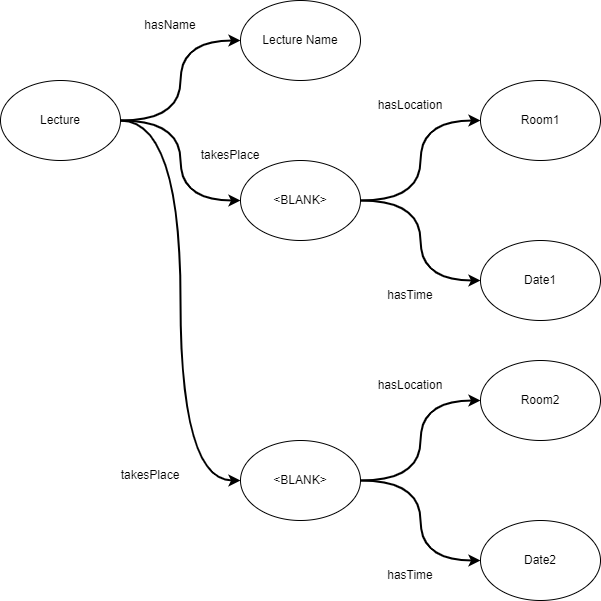
\includegraphics[width=0.6\textwidth]{./chapters/ch-semanticwebarchitecture/figures/lectureexp2.png}
	\caption{An example that demonstrate a lecture taking place at multiple locations and time slots using multi-valued relations and blank nodes.}
	\label{fig:lectureexp2}
\end{figure}

Turtle and other markup languages provides syntax for creating blank nodes that looks like the following.
\begin{lstlisting}
<subject1> <predicate1> [
	<predicate2> <object2>;
	<predicate3> <object3>
] .
\end{lstlisting}
To refer to a blank node, it is also possible to give the blank node a name. The syntax looks like the following.
\begin{lstlisting}
<subject1> <predicate1> _:<blank-node-name> .
_:<blank-node-name> <predicate2> <object2> .
_:<blank-node-name> <predicate3> <object3> .
\end{lstlisting}
where \verb|_:<blank-node-name>| is used to declare a blank node and assign it a name.

\subsection{Lists}

Lists help to make the code clean and readable. There are two types of lists, the container (open list, extendable) and the collections (closed list, fixed). Container is helpful to handle the situation given in Fig.  \ref{fig:lectureexp3}.
\begin{figure}[htbp]
	\centering
	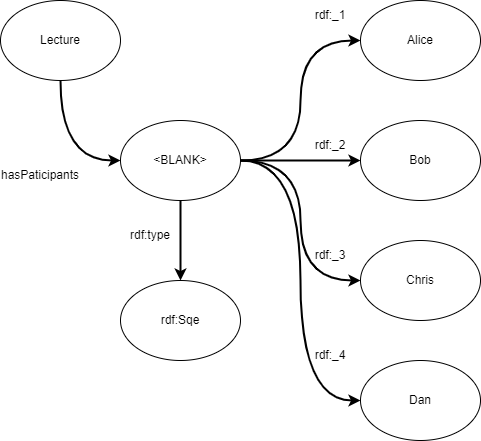
\includegraphics[width=0.6\textwidth]{./chapters/ch-semanticwebarchitecture/figures/lectureexp3.png}
	\caption{An example of a container.}
	\label{fig:lectureexp3}
\end{figure}
Notice that the blank node has a type \verb|rdf:Seq|. This tells that the items stored in the container follows an ordered set. There are other container types, such as \verb|rdf:Bag| (unordered set) and \verb|rdf:Alt| (alternatives of elements; only one element is relevant for the application).

The collection, on the other hand, defines a closed list as shown by Fig. \ref{fig:lectureexp4}. In turtle, this can be done by using nested \verb|[]| iteratively. 
\begin{figure}[htbp]
	\centering
	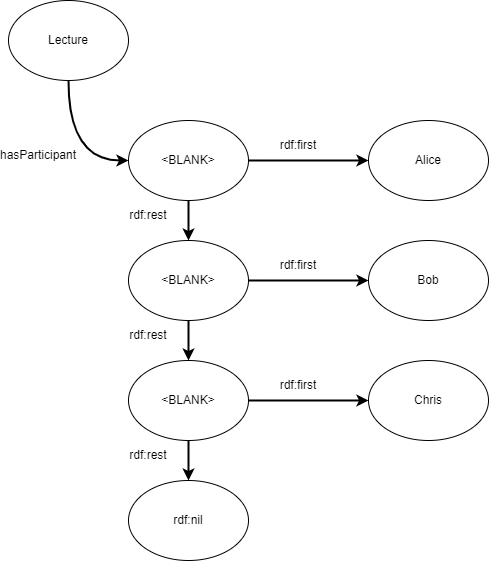
\includegraphics[width=0.6\textwidth]{./chapters/ch-semanticwebarchitecture/figures/lectureexp4.png}
	\caption{An example of a collection.}
	\label{fig:lectureexp4}
\end{figure}
A short cut is to use \verb|()|, with the items in the collection listed down in the bracket as follows.
\begin{lstlisting}
<subject> <predicate> (<object1> <object2> <object3>) .
\end{lstlisting}

\subsection{Reification}

RDF permits interleaving of statements, i.e., to make a statement about another statement. For example, consider ``Alice says that Bob ate the cake''. This example contains nested statement, where ``Bob ate the cake'' is a statement, and ``Alice says \ldots'' is a statement on that statement. RDF reification follows Fig. \ref{fig:reificationexp}.
\begin{figure}[htbp]
	\centering
	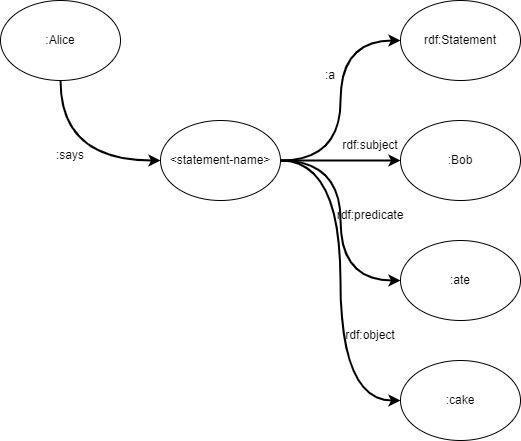
\includegraphics[width=0.6\textwidth]{./chapters/ch-semanticwebarchitecture/figures/reificationexp.png}
	\caption{An example of RDF reification.}
	\label{fig:reificationexp}
\end{figure}

\subsection{Converting RDB to RDF}

For small-scale relational database, it is possible to convert it to semantic web RDF manually. For example, consider an RDB for all the books in a study. There are three tables in the database, for books, authors and publishers, respectively. Each table contains a few dozens of entries. The RDB can be converted to RDF as shown in Fig. \ref{fig:bookexp}. It can be realized very easily, simply by defining everything as nodes and stack triples for all relationships. 
\begin{figure}[htbp]
	\centering
	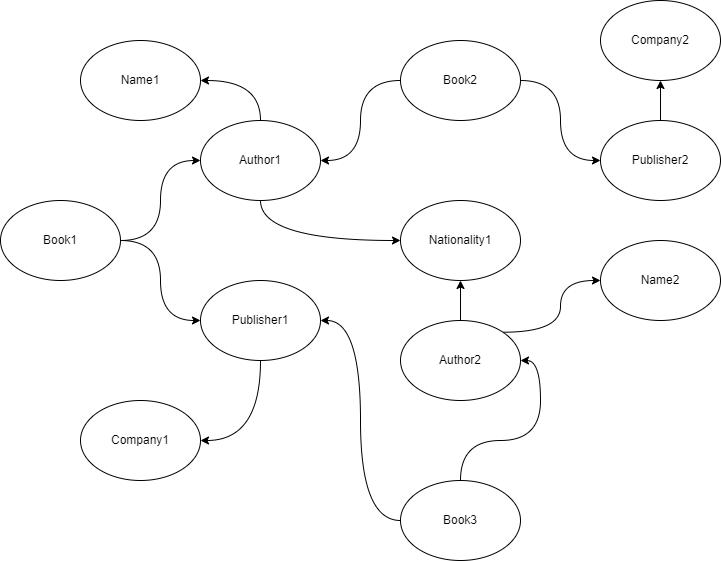
\includegraphics[width=0.8\textwidth]{./chapters/ch-semanticwebarchitecture/figures/bookexp.png}
	\caption{Semantic web of a few books, and their authors and publishers.}
	\label{fig:bookexp}
\end{figure}

However, when comes to a large and complicated database, converting it to RDF manually would consume too much labor. Several ways to systematically do the conversion have been proposed. Details are not covered here. See \cite{michel2014survey} for more details.

\subsection{Conclusion}

In summary, RDF, different from a plain XML or JSON which can also store independent classes, defines not only the objects (nodes) themselves but also the relationships among objects. This is essentially how RDF differs from a conventional key-value based NoSQL. RDF can be easily scaled up as nodes with the same name naturally merge together.

The underlying mechanism behind RDF, such as how machine stores graphical database including nodes and relationships, and how it enables query using SPARQL, is out of the scope of this notebook. In short, there are several ways to do that, for example by transforming the graph links into multiple small tables, etc. Different approaches may have their pros and cons. Details are neglected here.

\section{RDF Schema (RDFS)}

RDFS enforces schema to the RDF model. By using RDF/RDFS, a more consistent and semantic RDF model can be achieved compared with using RDF along.

\subsection{RDFS Motivation}

RDF is flexible. It is so flexible that sometimes it becomes difficult to maintain consistency of the RDF model, let alone performing sophisticated reasoning from it. RDFS, also known as RDF vocabulary description language, enforce schema to the RDF model by adding more ``meta information'' which builds more connections among the nodes.

RDFS expands the vocabulary of RDF. It introduces the concepts of ``class'' and ``subclass'' to RDF. It provides built-in predefined classes such as \verb|rdfs:Literal|, \verb|rdfs:Resource|, \verb|rdfs:Datatype|, etc., and enforce the nodes to be linked to these classes. RDF already defines \verb|rdf:Property|. RDFS further expands the properties and relations. All above makes the RDF modeling more consistent and semantic.

In the deeper insights, RDFS helps to add ``ontology'' to the RDF model by introducing the schema. It essentially integrate common understanding and domain knowledge to tine information. For example, by creating a property ``\verb|:hasSpouse|'' whose domain and range person, it demonstrates the common knowledge that a person can be married to another person.

\subsection{RDF Versus RDF/RDFS via an Example} \label{subsec:rdfvsrdfs}

The following example applies RDF versus RDF/RDFS on the same statement. Consider statement ``banana is yellow, apple is red, and orange is orange color''. In a RDF implementation, this would be simply be Fig. \ref{fig:fruitexp} green-colored elements. It is a disconnected graph, where the three statements are completely independent.
\begin{figure}[htbp]
	\centering
	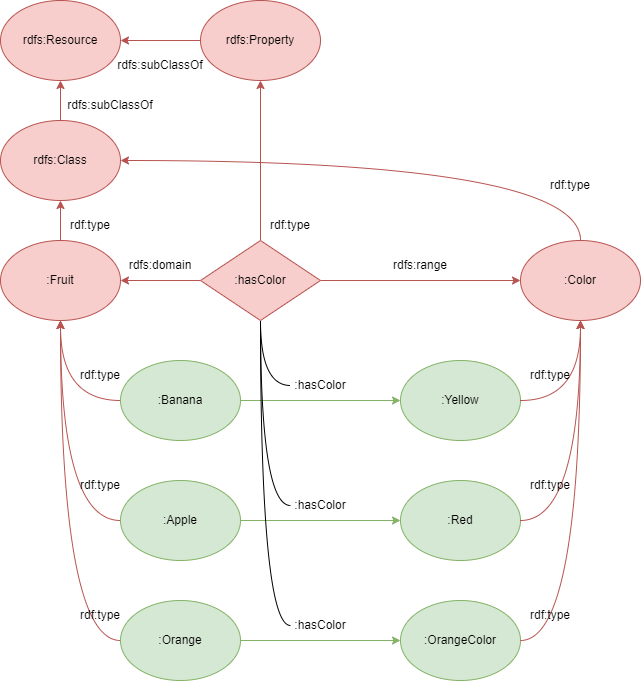
\includegraphics[width=0.8\textwidth]{./chapters/ch-semanticwebarchitecture/figures/fruitexp.png}
	\caption{Semantic web of a fruits, with the green color RDF and green + red RDF/RDFS implementations.}
	\label{fig:fruitexp}
\end{figure}

In a RDF/RDFS implementation, class/subclass and property are enforced in the RDF model, with property domain and range specified. All classes eventually root to \verb|rdfs:Resource|. This is shown by the green + red color in Fig. \ref{fig:fruitexp}. The corresponding Turtle is
\begin{lstlisting}
@prefix rdf: <http://www.w3.org/1999/02/22-rdf-syntax-ns#> .
@prefix rdfs: <http://www.w3.org/2000/01/rdf-schema#> .
@prefix example: <http://example.org/> .

# Define classes (optional; they are implicit)
rdfs:Class rdfs:subClassOf rdfs:Resource .
rdf:Property rdfs:subClassOf rdfs:Resource .

example:Fruit rdf:type rdfs:Class ;
rdfs:subClassOf rdfs:Resource .

example:Color rdf:type rdfs:Class ;
rdfs:subClassOf rdfs:Resource .

# Define properties
example:hasColor rdf:type rdf:Property ;
rdfs:domain example:Fruit ;
rdfs:range example:Color .

# Define fruits and colors
example:Banana rdf:type example:Fruit .
example:Apple rdf:type example:Fruit .
example:Orange rdf:type example:Fruit .

example:Yellow rdf:type example:Color .
example:Red rdf:type example:Color .
example:Green rdf:type example:Color .

# Define relationships between fruits and colors
example:Banana example:hasColor example:Yellow .
example:Apple example:hasColor example:Green .
example:Orange example:hasColor example:Orange .

\end{lstlisting} 
where only the last 3 lines would be used in RDF implementation. It can be seen from this example that RDF/RDFS uses more ``complicated'' structure to enforce schema of the model. In this example, ``a fruit has color of a color'' is enforced. Notice that predicate \verb|rdf:type| can be used interchangeably with turtle keyword \verb|a|. They both declares a instance of a class.

\subsection{RDFS Expanded Class and Properties}

Special classes and properties are defined, some of which already used in the above example. Some commonly seen ones include:
\begin{itemize}
	\item \verb|rdfs:Resource|
	\item \verb|rdfs:Class|
	\item \verb|rdf:Property|
	\item \verb|rdfs:subClassOf|
	\item \verb|rdfs:subPropertyOf|
	\item \verb|rdfs:domain|
	\item \verb|rdfs:range|
\end{itemize}

Commonly seen further properties of a node include the following. They help to make the RDF model more human-readable.
\begin{itemize}
	\item \verb|rdfs:seeAlso| points to a resource where a detailed explanation of the node can be found.
	\item \verb|isDefinedBy| defines the relation of a resource to its definition.
	\item \verb|rdfs:comment| points to text comment.
	\item \verb|rdfs:label| assign a more human-readable name to the node.
\end{itemize}

More details of the latest version of RDF/RDFS defined classes and properties are given by W3C and can be found at \textit{w3.org/TR/rdf-schema/}.

\subsection{Semantics inside RDF/RDFS}

The semantics in RDF/RDFS, such as Fig. \ref{fig:fruitexp}, is stored in the format of connections linked via properties, with domain and range specified. The name of a class or a property makes no sense to a machine when it is doing reasoning and query. The connection matters. 

The following gives some intuitive examples for semantic reasoning.
\begin{itemize}
	\item Via class inheritance. In Fig. \ref{fig:fruitexp}, if apple is a subclass of fruit, and fruit a subclass of plant, then apple must also be a subclass of a plant. There is an ``hidden arrow'' pointing from the apple to the plant.
	\item Via property domain and range. In Fig. \ref{fig:fruitexp}, if an unknown object ``hasColor'', then its object must be a fruit, and the subject a color. There are associated ``hidden arrows'', even if these arrows are not specified in the programming. 
	\item Via property inheritance. Consider two properties, ``isMotherOf'' and ``isParentOf''. Both properties have the same domain and range of ``person'', and ``isMotherOf'' is a sub property of ``isParentOf''. In this case ``A is the mother of B'' can derive ``A is the parent of B''. 
\end{itemize}

Though not given by the input directly, the hidden information exists in the semantic web and should be accessible from API

\section{SPARQL Protocol and RDF Query Language (SPARQL)}

SPARQL is the query language for semantic web. It is SQL-like in the API syntax perspective, but notice that the underlying technologies of SQL and SPARQL differ largely, as SQL is for operations on structured tabular, while SPARQL for those of graphical database. The details of the internal mechanism of SPARQL, which involves a lot of graph theory, pattern searching and data structuring, are not covered in this chapter.

In the recent update by W3C standard for SPARQL, namely SPARQL 1.1, more operations such as advanced query and interfering, updating triples, etc., have been added to the existing SPARQL 1.0 standard, making it more powerful and capable. SPARQL 1.1 is already supported by many triplestores. 

Notice that SPARQL is not only a language, but also a protocol layer. The input and return have specific formats which are also illustrated by the SPARQL standard. However, introducing of SPARQL from a protocol perspective is not the focus of this chapter, hence it is not covered in details. 

More details of SPARQL 1.1 can be found at \textit{w3.org/TR/sparql11-query/}.

\subsection{SPARQL for Basic Query}

Many query types are defined in SPARQL, each with a different purpose and associated with a different return type. For example,
\begin{itemize}
	\item SELECT returns a tabular just like SQL.
	\item CONSTRUCT returns a new RDF graph based on the query result.
	\item ASK returns true and false of whether a query has a solution.
	\item DESCRIBE returns the schematic of a resource; this is useful when the structure of RDF data in the data source is unclear.
\end{itemize}

The basic syntax of SPARQL is inspired by SQL as follows.
\begin{lstlisting}
SELECT [?s, ?p, ?o] 
[FROM rdfSource] 
WHERE {
	[?s/s] [?p/p] [?o/o]
}
[ORDER BY (?s/?p/?o)]
[LIMIT limitNum]
[PFFSET offsetNum]
\end{lstlisting}
where \verb|?variableName| denotes a variable, and without \verb|?|, a constant. Recall the fruit example used in Section \ref{subsec:rdfvsrdfs}. To perform a query to look for fruits with yellow color, use the following
\begin{lstlisting}
PREFIX ex: <http://www.example.com/>
PREFIX rdf: <http://www.w3.org/1999/02/22-rdf-syntax-ns#>

ASK WHERE {
	?fruit rdf:type ex:Fruit .
	?fruit ex:hasColor ex:Yellow .
} # return yes

SELECT ?fruit
WHERE {
	?fruit ex:hasColor ex:Yellow .
} # return a table with one element, ex:Banana

CONSTRUCT {?fruit ex:hasColor ?color}
WHERE {
	?fruit rdf:type ex:Fruit .
	?color rdf:type ex:Color .
	?fruit ex:hasColor ?color .
	FILTER (?color = ex:Yellow || ?color = ex:Red)
} # returns 2 triples, banana has color yellow and apple has color red

DESCRIBE ?fruit
WHERE {
	?fruit ex:hasColor ex:Yellow .
} # return triples related to ex:Banana
\end{lstlisting}

Always put in mind that SPARQL is essentially pattern matching. The triples given in the WHERE clause are the patterns to be matched. Only the elements or triples that matches all the patterns in the WHERE clause can be returned, on top of which other filtering functions (such as FILTER which is introduced later) can be carried out.

Notice that some triplestore may require each query to be passed to the engine one at a time, instead of putting everything into a gigantic file and ``run all''.

When there are string and numerical attributes, ``\verb|FILTER|'' keyword can be used to filter the result and returns only the entries matching the filter condition. An example is given below. It is worth mentioning that only triples in the WHERE clause need to end with a period ``.''. The filter condition lead by \verb|FILTER ()| does not require the period.
\begin{lstlisting}
PREFIX ex: <http://example.org/>

SELECT ?person 
WHERE {
	?person ex:age ?age .
	FILTER (?age >= 30 && ?age <= 40)
}
\end{lstlisting}

Commonly used keywords and operators in FILTER clause include \verb|&&| (and), \verb$||$ (or), \verb|!| (not), as well as string functions \verb|STR|, \verb|LANG|, \verb|CONTAINS|, \verb|STRSTARTS|, \verb|STRENDS|, \verb|STRLEN|, \verb|SUBSTR|, \verb|REGEX| (regular expression matching), etc., and numeric functions \verb|+|, \verb|-|, \verb|*|, \verb|/|, \verb|>|, \verb|>=|, \verb|<|, \verb|<=|, \verb|ABS|, \verb|ROUND|, \verb|CEIL|, \verb|FLOOR|, etc., and comparison operators \verb|=|, \verb|!=|.

Similar with FILTER clause, there are also other clauses such as OPTIONAL, UNION, etc. The OPTIONAL clause indicates that if the entry does not have the attribute to be evaluated in the clause, it still passes the query. An example of is given below, where RDF and SPARQL are given separately. RDF:
\begin{lstlisting}
@prefix foaf: <http://xmlns.com/foaf/0.1/> .

:alice
a foaf:Person ;
foaf:name "Alice" ;
foaf:mbox <mailto:alice@example.com> .

:bob
a foaf:Person ;
foaf:name "Bob" .
\end{lstlisting}
SPARQL:
\begin{lstlisting}
PREFIX foaf: <http://xmlns.com/foaf/0.1/>

SELECT ?name ?email
WHERE {
	?person a foaf:Person ;
	foaf:name ?name .
	OPTIONAL { ?person foaf:mbox ?email . }
}
\end{lstlisting}
The above returns both names and Alice's email, and it won't fail although Bob does not have an attribute of email.

The UNION clause allows the combination of two queries as one return, given that the structure of the queries matches. An example is given below.
\begin{lstlisting}
PREFIX foaf: <http://xmlns.com/foaf/0.1/>
SELECT ?name 
WHERE {
	{
		?person a foaf:Person .
		?person foaf:name ?name .
	} 
	UNION 
	{
		?organization a foaf:Organization .
		?organization foaf:name ?name .
	}
}
\end{lstlisting}
which would return both people and company names in one go.

\subsection{SPARQL for Advanced Operations}

SPARQL 1.0 provides basic query functions based on graph pattern matching, as already explained in the previous section. SPARQL 1.1 provides advanced query functions as follows.

\vspace{0.1in}
\noindent \textbf{Advanced Query}
\vspace{0.1in}

In the SELECT clause, it allows simple calculations on top of the returned result, and name it as a new column. For example,
\begin{lstlisting}
SELECT ?x (?y*1.1 AS ?z)
WHERE {
	?x ex:hasProperty ?y .
}
\end{lstlisting}
returns \verb|?y*1.1| instead of \verb|?y|, and furthermore rename it as \verb|?z|.

SPARQL 1.1 enables aggregate functions. For example,
\begin{lstlisting}
PREFIX ex: <http://www.example.com/>
PREFIX rdf: <http://www.w3.org/1999/02/22-rdf-syntax-ns#>

SELECT (Count(?fruit) AS ?numOfFruit)
WHERE {
	?fruit rdf:type ex:Fruit .
}

SELECT (Count(DISTINCT ?fruit) AS ?numOfFruit)
WHERE {
	?fruit rdf:type ex:Fruit .
}
\end{lstlisting}
counts the total number of fruits in the database. Notice that when using aggregate functions, new variable name (in this example, \verb|?numOfFruit|) must be assigned. Otherwise, there will be an syntax error.

\vspace{0.1in}
\noindent \textbf{Data Editing}
\vspace{0.1in}

SPARQL provides operations to insert, edit, and delete elements in a semantic web as follows.
\begin{itemize}
	\item INSERT inserts triples into a graph.
	\item DELETE deletes triples from a graph.
\end{itemize}

Recall the fruit example used in Section \ref{subsec:rdfvsrdfs}. To create that RDF/RDFS database from scratch using SPARQL, use the following (notice that ``orange is orange color is changed to pear is green'')
\begin{lstlisting}
PREFIX ex: <http://www.example.com/>
PREFIX rdfs: <http://www.w3.org/2000/01/rdf-schema#>
PREFIX rdf: <http://www.w3.org/1999/02/22-rdf-syntax-ns#>

INSERT DATA {
	# Define resources
	ex:Banana rdf:type ex:Fruit .
	ex:Apple rdf:type ex:Fruit .
	ex:Pear rdf:type ex:Fruit .
	ex:Yellow rdf:type ex:Color .
	ex:Red rdf:type ex:Color .
	ex:Green rdf:type ex:Color .
	
	# Define properties
	ex:hasColor rdf:type rdf:Property ;
	rdfs:domain ex:Fruit ;
	rdfs:range ex:Color .
	
	# Link resources with properties
	ex:Banana ex:hasColor ex:Yellow .
	ex:Apple ex:hasColor ex:Red .
	ex:Pear ex:hasColor ex:Green .
}
\end{lstlisting}

\subsection{Default Graph and Named Graph}

It is worth mentioning that it is possible to create and query ``disjoint'' graphs using SPARQL. If the graph name is not specified during the inserting of the data, the data is inserted into the default graph. A query can have multiple FROM clause, each specifying a graph. If the graph name is not specified during the query, all graphs will be searched. An example of inserting and querying named graph is given below.

\begin{lstlisting}
INSERT DATA {
	GRAPH <http://example.org/mygraph> { 
		<http://example.org/book1> <http://purl.org/dc/elements/1.1/title> "A new book" .
	}
	GRAPH <http://example.org/myothergraph> { 
		<http://example.org/book2> <http://purl.org/dc/elements/1.1/title> "Another book" .
	}
}

SELECT ?book ?title WHERE {
	GRAPH <http://example.org/mygraph> {
		?book <http://purl.org/dc/elements/1.1/title> ?title .
	}
}
\end{lstlisting}

The relationship of the graphs is somehow like the different tables in an RDS. They usually represent logically separated things, but they can have some overlaps. When doing analysis information can be extracted from multiple graphs at the same time.

\subsection{SPARQL Returns}

As introduced earlier, SPARQL is an HTML based protocol. The returned result of a SPARQL query can be specified in the HTML header. There are several return types defined in the standard. When SELECT or ASK are used, the return types can be:
\begin{itemize}
	\item XML
	\item JSON
	\item TSV (table-separated values, similar to CSV)
\end{itemize}
When CONSTRUCT or DESCRIBE are used, the return is an RDF that can be in 
\begin{itemize}
	\item RDF/XML
	\item Turtle
	\item N-Triples
	\item JSON-LD
\end{itemize}
and a few more. The decoding of the return can be done my relative tools and packages, and are not given in details here.

\section{A Bit More Insights on RDF/RDFS}

RDF can be represented as a set of triples, which makes it readable for both humans and machines. When using SPARQL to query or edit RDF database, RDF is treated as directional graphs with some sort of hierarchy. This is the interface of RDF database, following W3C standard.

How about the underlying data structure that ultimately supports the interface, making sure that everything runs smoothly and efficiently?

Different triplestores may have different preference when choosing the underlying data structure.

\section{Web Ontology Language (OWL)}

By adding schema to RDF, RDFS already boosts the capability and adds ontology to the RDF model. However, there are still a number of limitations using RDF/RDFS alone.

\subsection{OWL Motivation}

OWL provides additional features to enforce and enhance the schema of an RDF model. 

It provides different levels of  ``consistency checks'' and applies ``limitations'' to the classes and instances in an RDF model. It adds identity equivalence and difference features by introducing properties such as \verb|sameAs|, \verb|differentFrom|, \verb|equivalentClass|, \verb|equivalentProperty|. It offers more expressive class definitions including intersection, union, complement and disjointness of classes. It further enlarge the vocabulary sets of the RDF model.

\section{Commonly Used Namespace}

Commonly used built-in name spaces are summarized in Table \ref{tab:commonnamespace}.

\begin{table}
	\centering \caption{Commonly used namespaces in RDF models.} \label{tab:commonnamespace}
	\begin{tabularx}{\textwidth}{|c|c|X|}
		\hline
		Namespace & URI & Description \\ \hline
		\verb|foaf| & \verb|http://xmlns.com/foaf/0.1/| & Friend-of-a-friend. It describes people, their activities and relations to other people and object. \\
		\hline
	\end{tabularx}
\end{table}



